\documentclass[dvipdfmx]{jarticle}
\usepackage{graphicx}
\usepackage[top=30truemm,bottom=30truemm,left=25truemm,right=25truemm]{geometry}
\usepackage{listings,jvlisting}
\usepackage{url}
\usepackage{tikz}
\usetikzlibrary{shapes.geometric, arrows}

\tikzstyle{startstop} = [rectangle, rounded corners, minimum width=3cm, minimum height=1cm, text centered, draw=black, fill=red!30]
\tikzstyle{process} = [rectangle, minimum width=3cm, minimum height=1cm, text centered, draw=black, fill=orange!30]
\tikzstyle{decision} = [diamond, minimum width=3cm, minimum height=1cm, text centered, draw=black, fill=green!30]
\tikzstyle{arrow} = [thick,->,>=stealth]

\begin{document}
\begin{titlepage}
    \begin{center}
        {\huge 情報科学演習C 課題2レポ―ト}
        \vspace{180pt}\\
        \begin{tabular}{rl}
            氏名 & 山久保孝亮\\
            所属 & 大阪大学基礎工学部情報科学科ソフトウェア科学コース\\
            メールアドレス & u327468b@ecs.osaka-u.ac.jp\\
            学籍番号 & 09B22084\\
            提出日 & \today\\
            担当教員 & 平井健士,中島悠太
        \end{tabular}
    \end{center}
\end{titlepage}
\section{課題2-1}
\subsection{アルゴリズム}
今回私が作成したechoclientプログラムは以下の図1ようなフローチャートとなる.
\begin{figure}[h]
    \center
    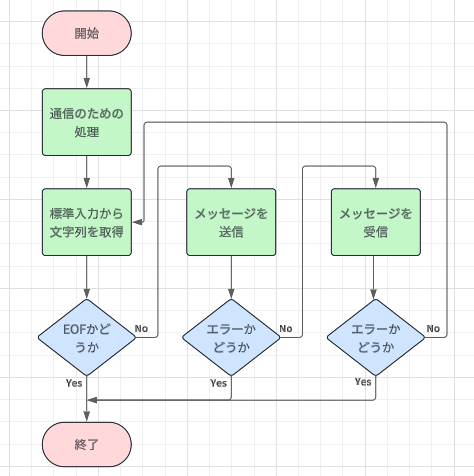
\includegraphics[width=8cm]{hurotya1.png}
    \caption{echoclientプログラムのフローチャート}
\end{figure}
\\また,通信のための処理の内容は以下の通りとなる
\begin{enumerate}
    \item 入力形式の確認
    \item ソケットの生成
    \item ホストが存在するかどうかを確認
    \item ソケットアドレス再利用の指定
    \item ソケット接続先の情報設定
    \item ソケットをサーバーに接続
\end{enumerate}
以下でその詳細について述べる.
\subsubsection{入力形式の確認}
今回のechoclientプログラムは第一引数としてホスト名を指定するという使用法を想定している.そのため,それ以外の使用を制限するために
main関数のコマンドライン引数であるargcの値を確認することで実現した.argcは指定した引数の個数+1の値を表すのでこれが2出ない場合は正しい書式でないとして
エラーメッセージを表示し,プログラムを終了する.
\subsubsection{ソケットの生成}
ソケットを生成するには,socketシステムコールを使用する.今回はUDPを使用するので第一引数にはAF\_INET,第二引数にはSOCK\_DGRAM,第三引数には0を指定した.第三引数に0を指定するとドメインの種類とソケットの型によってデフォルトのプロトコルが選ばれる.\cite{2}
socketシステムコールは正常に実行された場合は負でないソケット記述子を返し,以上があれば-1を返す.そのため,正常に終了したかどうかを確かめるために返り値を格納するint型変数sockの値が0より小さいかどうかを条件分岐で判定する.
正常に実行されていなければエラーメッセージを出力しプログラムを終了する.
\subsubsection{ホストが存在するかどうかを確認}
ホストが存在するかどうかを確認するためにgethostbynameシステムコールを使用した.引数は一つでホスト名を指す文字列で,正常終了するとhostent構造体へのポインタを返し,エラーが発生した場合はNULLを返す.\cite{1}
したがって,hostent構造体の構造体変数のポインタとしてserverを定義し,これにgethostbynameシステムコールの返り値を格納した.また,引数にはコマンドライン引数のargv[1]を使用した.
その後gethostbynameシステムコールが正常に終了したかどうかを判定するためにserverにNULLポインタが返されていないかを条件分岐によって確認する.もし返されていればエラーメッセージを出力しプログラムを終了する.
\subsubsection{ソケットアドレス再利用の指定}
setsockopt関数を使ってソケット関連のオプションを設定する.引数は5つあり,いかにその詳細を記述する.\cite{3}\cite{4}
\begin{itemize}
    \item 第一引数:オプションの適用先であるソケット
    \item 第二引数:オプションが設定しているレベル.様々なレベルがあるが,SOL\_SOCKETは第一引数で指定したソケットのオプションのレベルが得られる.
    \item 第三引数:指定するソケットオプションの名前.様々なオプションがあるが,今回使用するSO\_REUSEADD\\Rについて記述する.これは通常一定時間ほかのソケットがそのポートを使えなくなってしまうことを防ぐことができるようになる.\cite{5}
    \item 第四引数:オプションデータへのポインタ.SO\_RESUSEADDRを有効にするには整数型で1の値が渡される.
    \item 第五引数:オプションデータの長さ.
\end{itemize}
また,返り値は正常に実行された場合は0を返し,されなかった場合は-1を返す.したがって,今回作成したプログラムではint型変数reuseを1に設定し,setsockopt関数の引数に使用して正常に実行されたかを確認するために返り値が0未満かどうかで条件分岐をさせた.
正しく実行されていなかった場合はエラーメッセージを出力しプログラムを終了した.
\subsubsection{ソケット接続先の情報設定}
ここでは,hostnet構造体とsockaddr\_in構造体のメンバに情報を格納している.sockaddr\_in構造体のメンバは以下のようになっている.\cite{6}\cite{7}
\begin{itemize}
    \item sin\_len:sin\_addrの変数のサイズ
    \item sin\_family:アドレスファミリを指定
    \item sin\_port:ポート番号を指定
    \item in\_addr sin\_addr:IPアドレスをin\_addr構造体で指定
    \item sin\_zero[8]:OSの内部仕様専用
\end{itemize}
sockaddr\_in構造体の構造体変数名はsvrとした.以下のプログラムのように情報を設定した.
1行目ではsvrのすべてのメンバをbzero関数を使ってゼロに初期化している.2行目はsvrのメンバsin\_familyにAF\_INETを設定している.
3行目ではサーバーのIPアドレスを1.1.5で取得し,serverのメンバに格納されているサーバーのIPアドレスをsvrのメンバにbcopy関数を使ってコピーする.4行目ではsvrのメンバにポート番号を指定している.
\subsubsection{ソケットをサーバーに接続}
ここではconnectシステムコールを使ってソケットをサーバに接続している.connectシステムコールの引数は以下のようになる.\cite{8}
\begin{itemize}
    \item socket:ソケット記述子
    \item address:接続試行先のsockaddr構造体へのポインター
    \item address\_len:addressパラメータがさすsockaddr構造体のサイズ
\end{itemize}
また,返り値は正常に終了した場合は0を,異常が発生すると-1を返す.
今回のプログラムでは第一引数にsock,第二引数にsvrへのポインタ,第三引数にsvr構造体の長さを格納している.そして
connectシステムコールの返り値が0より小さければ異常が発生したとしてソケットを閉じてプログラムを終了する.
\subsubsection{繰り返し処理}
今回のプログラムの仕様では標準入力から読み込んだ文字列をサーバプログラムへ送信し受信した文字列をEOFを受け取るまで繰り返すというものであった.
したがって,以下の1.1.8と11.9で記述するメッセージの送信と受信はEOFが入力されるまで繰り返し実行される必要があるから,while文を使ってそれらの処理を無限ループにした.
つまり,各ループごとにユーザにfgets関数を使って標準入力から文字列を配列rbufに格納し,それをサーバに送信,受信するというアルゴリズムを採用した.
\subsubsection{メッセージをサーバーに送信}
ここではwriteシステムコールを使ってソケットにデータを送信している.writeシステムコールの引数は以下のようになる.\cite{9}
\begin{itemize}
    \item fs:ソケット記述子
    \item buf:書き込まれるデータを保留するバッファを指すポインタ
    \item n:bufパラメータが指すバッファの長さ
\end{itemize}
返り値は,正常に実行されたときは0以上の値を返し正常に実行されなかった場合は-1を返す.
fsにはsock,bufにはrbuf,nにはstrlen関数を使って取得したbufの長さを設定した.そして変数nにwriteシステムコールの返り値を格納する.
nが0より小さければ異常に終了したと判定しソケットを閉じてプログラムを終了する.
\subsubsection{メッセージをサーバーから受信}
ここではreadシステムコールを使ってソケットからデータを読み取っている.readシステムコールの
引数は以下のようになる.\cite{10}
\begin{itemize}
    \item fs:ファイルまたはソケットの記述子
    \item buf:データを受け取るバッファへのポインタ
    \item n:bufパラメータがさすバッファの長さ
\end{itemize}
返り値は,正常に実行されたときは読み込んだバイト数を,異常終了した場合は-1を返す.\cite{11}
今回のプログラムではfsにsock,bufにrbuf,nにはstrlen関数を使って取得したbufの長さを設定した.
そして変数nにreadシステムコールの返り値を格納する.
nが0より小さければ異常に終了したと判定しソケットを閉じてプログラムを終了する.
\subsection{実行結果}
以下の図2と図3はechoserverとechoclientを実行し,文字列"aiueo"を入力したときの動作結果を表している.
\begin{figure}[htbp]
    \begin{minipage}[b]{0.45\linewidth}
      \centering
      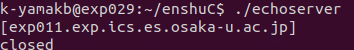
\includegraphics[keepaspectratio, scale=0.5]{2-1server.png}
      \caption{echoserverの実行結果}
    \end{minipage}
    \begin{minipage}[b]{0.45\linewidth}
      \centering
      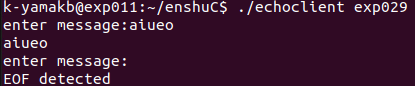
\includegraphics[keepaspectratio, scale=0.5]{2-1client.png}
      \caption{echoclientの実行結果}
    \end{minipage}
\end{figure}
\\echoserverはexp029というホストで,echoclientはexp011というホストでプログラムを実行した.仕様のとおり,client側から文字列を入力すると改行されて正しく同じ文字列が表示されていることがわかる.
そして最後にEOFを入力するとサーバとの接続が終了している.
\section{課題2-2}
\subsection{simple-talk-serverのアルゴリズム}
今回私が作成したsimple-talk-serverプログラムのフローチャートは以下の図4のようになる.
\begin{figure}[h]
    \center
    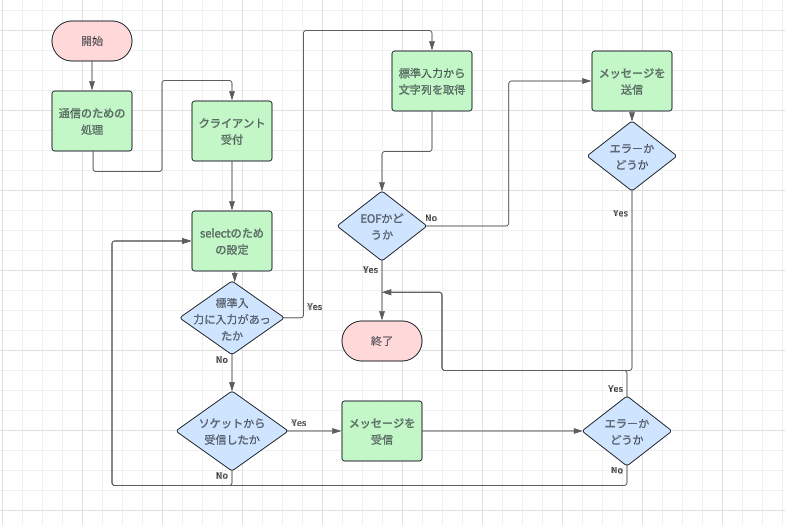
\includegraphics[width=8cm]{hurotyaserver.png}
    \caption{simple-talk-serverプログラムのフローチャート}
\end{figure}
\\simple-talk-serverの通信のための処理は以下のとおりである.
\begin{enumerate}
    \item ソケットの生成(1.1.2と同様)
    \item ソケットアドレスの再利用の指定(1.1.4と同様)
    \item クライアント受け付け用ソケットの情報設定
    \item ソケットアドレスの割り当て
    \item 待ち受けクライアント数の設定
\end{enumerate}
以下でその詳細について述べる.
\subsubsection{クライアント受付用ソケットの情報設定}
基本的には1.1.5で述べた内容と同じであるが,このプログラムの3行目ではサーバ側のIPアドレスを指定している.
htonl関数は引数がホストバイトオーダーで表現された32ビット数で,返り値はTCP/IPネットワークバイト順で値を返す.\cite{12}INADDR\_ANYとするとサーバは全ての利用可能なインターフェースからの接続を受け付けるということを意味する.\cite{13}
\subsubsection{ソケットアドレスの割り当て}
ここではbindシステムコールを使用してソケットをサーバのアドレスにバインドしている.
bindシステムコールの引数は以下のようになる.\cite{14}
\begin{itemize}
    \item sockfd:ファイルディスクリプタ
    \item addr:sockaddr構造体のポインタで関連付けるアドレス情報を保持
    \item addrlen:addrのアドレス構造体のサイズを指定
\end{itemize}
返り値は正常に実行されると0が返され,エラーが発生した場合は-1が返される.今回のプログラムでもsockaddr\_in構造体の構造体変数名をsvrとしているため,第一引数に2.1.2で取得したsock,第二引数にsvrのアドレス,第三引数にsvrのアドレスのサイズ
を指定している.エラーを検出するためにbind関数の返り値が0より小さいときにはプログラムを終了する.
\subsubsection{待ち受けクライアント数の設定}
ここではlistenシステムコールを実行してソケットを接続待ちソケットとする.\cite{15}引数は以下の2つである.
\begin{itemize}
    \item sockfd:ファイルディスクリプタ
    \item backlog:sockfdについての保留中の接続のキューの最大長
\end{itemize}
返り値は成功した場合は0が返され,エラー時には-1が返される.今回のプログラムでは第一引数に1.1.2で取得したsock,第二引数には5を指定する.エラーを検出するためにlisten関数の
返り値が0より小さいときにはプログラムを終了する.
\subsubsection{クライアント受付}
1行目ではsvrとは別に定義されたsockaddr\_in構造体の構造体変数であるcltを使用してcltのサイズをclenに格納する.これは,cltが接続してきたクライアントのアドレス情報を格納するためのものであるからである.
2行目ではacceptシステムコールの返り値をcsockに格納する.1.1.2で取得したsockではなくcsockを使う理由は,acceptは待ち受けている接続要求の一つを受け入れ,新しいファイルディスクリプタを返すためである.
acceptシステムコールの引数は以下のとおりである.
\begin{itemize}
    \item s:listenシステムコールによって待ち受け状態となっているソケットを識別するファイルディスクリプタ
    \item sockaddr *addr:通信相によって認識されている接続中エントリのアドレスウを受け取るバッファへのポインタ
    \item *addrlen:addrパラメータがさす構造体の長さを指す変数へのポインタ
\end{itemize}
返り値は成功したときは新しいソケットのファイルディスクリプタを,失敗すると-1を返す.したがって,失敗したかどうかを判定するためにaccept関数の返り値が格納されているcsockが0より小さい時にはプログラムを終了する.
\subsubsection{クライアントのホストの情報取得}
ここではgethostbyaddr関数を使ってIPアドレスからホスト情報を逆引きしている.これにより,2.1.6で受け付けたクライアントの情報を取得する.また,ここまで処理が進めばクライアント側と接続したことになるので"Connected with (クライアント側のホスト名)"を出力する.
\subsubsection{selectのための設定}
今回のプログラムの仕様では,サーバ側もクライアント側も標準入力に入力があった時とメッセージを相手側から受信したときとで処理する内容が違っていた.この機能を実現するためにselectシステムコールを使用した.これを使うことによりファイルディスクリプタの状態の変化を監視することができる.

ここではselectシステムコールを使うための設定を行っている.
1行目のFD\_ZEROはfd\_set型のrfdsを空集合にするマクロで,2,3行目のFD\_SETはファイルディスクリプタである0とcsockをrfdsに追加している.ファイルディスクリプタを0にすると,標準入力であることを表す.\cite{16}
これにより,標準入力空の入力があるかどうかとクライアントソケットからのデータ受信を監視できるようになる.
4から5行目では監視する待ち時間をtimeval構造体のメンバの値に設定している.timeval構造体のメンバは以下のとおりである.
\begin{itemize}
    \item tv\_sec:指定する時間の1秒以上の部分
    \item tv\_usec:指定する時間の1秒未満の部分
\end{itemize}
即ち,今回のプログラムでは構造体変数名をtvとして待ち時間を1秒に指定している.
\subsubsection{繰り返し処理}
selectシステムコールの引数は以下のとおりである.\cite{1}
\begin{itemize}
    \item 監視するファイルディスクリプタの最大値に1を加えた整数.NULLポインタを入れると監視しない
    \item 読み込みを監視するファイルディスクリプタの集合.NULLポインタを入れると監視しない
    \item 書き込みを視するファイルディスクリプタの集合.NULLポインタを入れると監視しない
    \item 例外発生視するファイルディスクリプタの集合.NULLポインタを入れると監視しない
    \item selectを監視する待ち構造体timevalへのポインタ.NULLを指定すると監視するファイルディスクリプタのいずれかの状態が変化するまで無期限にブロックする.
\end{itemize}
監視しない項目はNULLポインタを入れる.返り値は状態が変化したファイルディスクリプタの総数または-1を返す.
今回のプログラムでは引数をcsock+1,rfdsのアドレス,NULL,NULL,tvのアドレスを指定している.selectが0より大きい値を返す時には標準入力または読み込み可能なファイルディスクリプタが存在し,0以下であれば
タイムアウトが発生したことを表し,これを無限ループの中に入れることによって常に監視し続けることができる.
\subsubsection{メッセージをサーバーに送信}
FD\_ISSETを使って0がrfdsに入っているかどうかを判定する.入っていない場合は0を返し,入っている場合はそれ以外の値を返す.\cite{17}
基本的な処理内容は1.1.8と同じであるが,エラーが発生した場合はソケットをcloseしてプログラムを終了するようにする.
\subsubsection{メッセージをサーバーから受信}
FD\_ISSETを使ってcsockがrfdsに入っているかどうかを判定する.
基本的な処理内容は1.1.9と同じであるが,エラーが発生した場合はソケットをcloseしてプログラムを終了するようにする.
\subsection{simple-talk-clientのアルゴリズム}
今回私が作成したsimple-talk-serverプログラムのフローチャートは以下の図5のようになる.
\begin{figure}[h]
    \center
    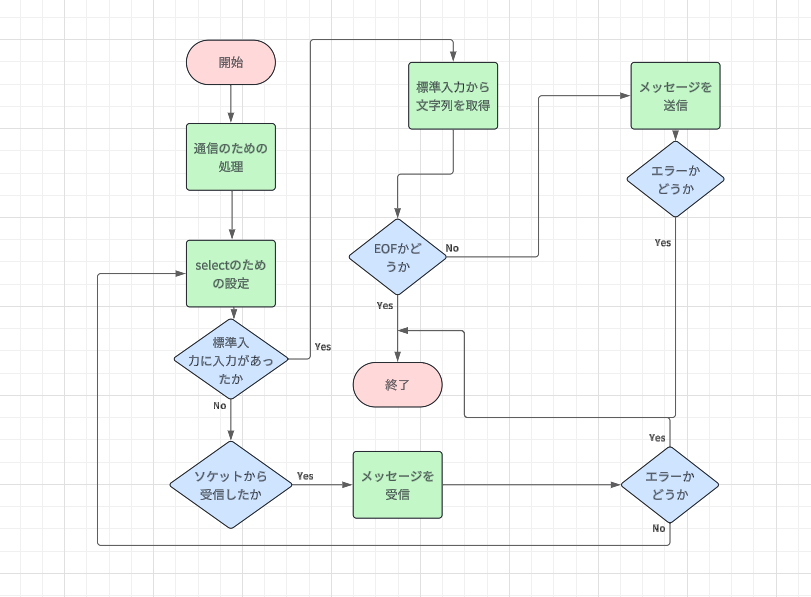
\includegraphics[width=8cm]{hurotyaclient.png}
    \caption{simple-talk-clientプログラムのフローチャート}
\end{figure}
また,simple-talk-clientの通信のための処理は以下のとおりである.
\begin{enumerate}
    \item 書式の確認
    \item ソケットの生成(1.1.2と同様)
    \item ホストが存在するかどうかを確認
    \item ソケットアドレス再利用の指定(1.1.4と同様)
    \item サーバ受付用アドレスの設定(1.1.5と同様)ただし,ポート番号は10130とした.
    \item ソケットをサーバに接続(1.1.6と同様)
\end{enumerate}
また,selectのための処理以降はsimple-talk-serverと同じ処理である.
以下では,simple-talk-serverとは異なっている1と3内容の詳細を記述する.
\subsubsection{書式の確認}
このプログラムは引数にホストを持つので,コマンドライン引数の長さであるargcを使って引数の個数による条件分岐を作成した.正しい書式である,argcが2の時以外は
プログラムを終了するものとした.
\subsubsection{ホストが存在するか確認}
ここでは,第一引数で指定したホストが存在するかをgethostbynameシステムコールを使って確認している.1.1.3で述べたように,正常終了すると返り値としてhostent構造体へのポインタを返し,エラーが発生したときは
NULLを返すので返り値を格納している変数serverがNULLかどうかの条件分岐を作成し,エラーの場合即ち引数で指定したホストが見つからない場合はプログラムを終了する.
\subsection{実行結果}
以下の図6と図7はsimple-talk-serverとsimple-talk-clientを実行し,サーバから文字列"aiueo"を,クライアントから文字列"kakikukeko"を入力したときの動作結果を表している.
\begin{figure}[htbp]
    \begin{minipage}[b]{0.45\linewidth}
      \centering
      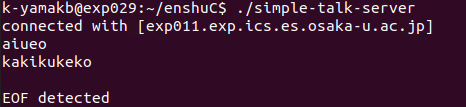
\includegraphics[keepaspectratio, scale=0.5]{2-2server.png}
      \caption{simple-talk-serverの実行結果}
    \end{minipage}
    \begin{minipage}[b]{0.45\linewidth}
      \centering
      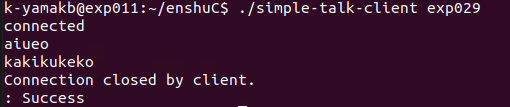
\includegraphics[keepaspectratio, scale=0.5]{2-2client.png}
      \caption{simple-talk-clientclientの実行結果}
    \end{minipage}
\end{figure}
\\echoserverはexp029というホストで,echoclientはexp011というホストでプログラムを実行した.仕様のとおり,お互いの文字列を正しく表示していることがわかる.
そして最後にEOFを入力するとサーバとの接続が終了している
\section{発展課題}
\subsection{lowerechoserverの作成}
echoserverのコードの一部を書き換えて実装した.
受信した文字列中のすべての大文字を小文字に変換するためにctype.hというインクルードファイルをインクルードし,writeシステムコールの直前で受信した文字列が格納されているrbufの各要素に対して
tolower関数を適用しその返り値を変換した後の文字列を格納する配列lbufに格納する.これはwhile分の繰り返しにより行われ,繰り返しの条件はrbufの要素がヌル文字であるかどうかである.
ヌル文字であれば繰り返しを終了し,lbufの次の要素の内容をヌル文字にし,writeシステムコールによってlbufを出力する.以下の図8と図9はlowerechoserverとechoclientを実行し,クライアントから文字列
"aiueo"と"Aiueo"を入力したときの動作結果を表している.
\begin{figure}[htbp]
    \begin{minipage}[b]{0.45\linewidth}
      \centering
      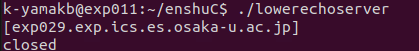
\includegraphics[keepaspectratio, scale=0.5]{3-1server.png}
      \caption{lowerechoserverの実行結果}
    \end{minipage}
    \begin{minipage}[b]{0.45\linewidth}
      \centering
      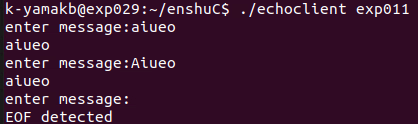
\includegraphics[keepaspectratio, scale=0.5]{3-1client.png}
      \caption{echoclientの実行結果}
    \end{minipage}
\end{figure}
\\echoserverはexp011というホストで,echoclientはexp029というホストでプログラムを実行した.仕様のとおり,client側から文字列を入力すると大文字を小文字に変換して正しく同じ文字列が表示されていることがわかる.
そして最後にEOFを入力するとサーバとの接続が終了している.
\subsection{起こりうる例外的な動作}
このプログラムはsimple-talk-server-2という名前で作成した.
simple-talk-serverにおいて,一つのサーバに複数のクライアントが接続しようとしたときには,最初に接続されたクライアントとの接続は継続し,それ以外のクライアントからの受付は拒否するという仕様に変更することによって
この例外的な動作へのエラー処理を実現した.
具体的な実装方法としては,selectシステムコールに新しい接続要求があったかどうかを判定する条件分岐を追加して検出し,現在混んでいるという文字列を新たに接続しようとしてきたクライアントに対して送信する.
以下の図10はexp039がサーバであるexp037と接続した後にさらにexp040がサーバに接続しようとした様子を示している.
\begin{figure}[h]
    \centering
    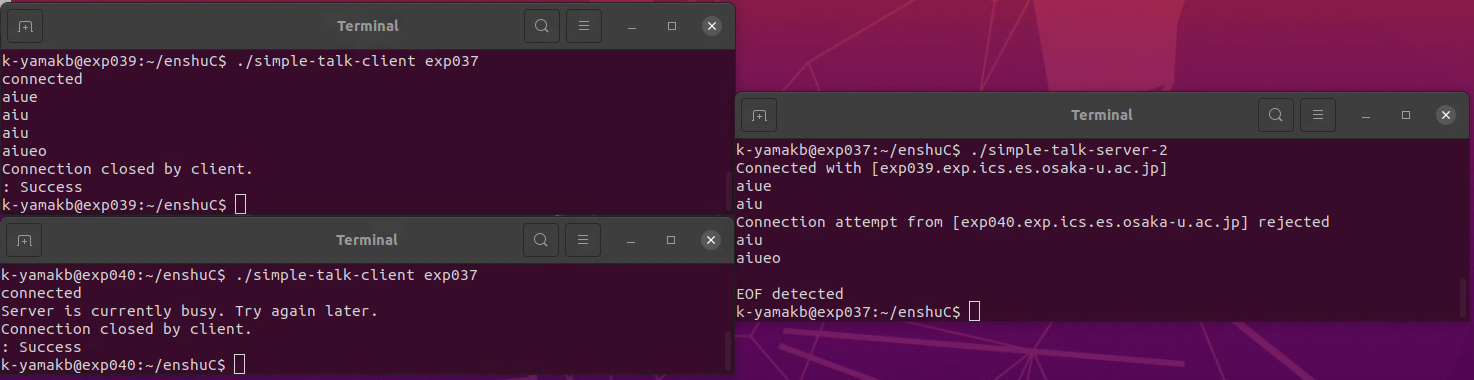
\includegraphics[width=12cm]{3-2.png}
    \caption{実行結果}
\end{figure}

上図から分かるように,接続要求を出したクライアントには現在混みあっているという文字列が表示され,サーバにはどのクライアントから接続要求があったのかが表示される.また,この接続の拒否が起こった後でも
課題2のようにメッセージの送受信は正常に実行されているb.
\subsection{課題2-2のプログラムの改良}
このプログラムはsimple-talk-server-3,simple-talk-client-3という名前で作成した.
メッセージに誰の発言かを表示させるために送信するメッセージの内容に送り主のホスト名を追加するという方針で実装した.
具体的には,hostnameという配列を用意し,gethostname関数を使ってhostnameに自分のホスト名を格納する.そして送信する際の処理のところで,fgets関数によってメッセージが格納されたrbufとhostnameをsnprintf関数を使って
"[ホスト名]:メッセージの内容"の形で結合した文字列を配列sbufに格納する.このsbufをwriteシステムコールで送信することにより使用を実現した.これはクライアント側もホスト側も同じように実装した.
\begin{figure}[h]
    \centering
    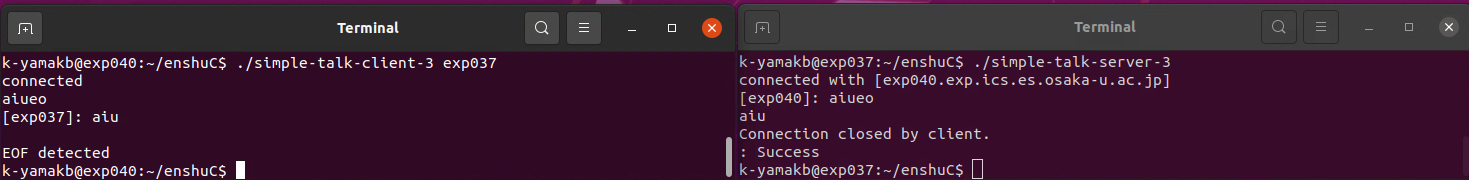
\includegraphics[width=12cm]{3-3.png}
    \caption{実行結果}
\end{figure}
\\
図11から分かるようにホストexp037がサーバプログラムを,ホストexp040がクライアントプログラムを実行しており,双方向からのメッセージは受信したときにはお互いのホスト名を表示していることがわかる.
\section{感想}
今回の課題を通してUDP及びTCPへの理解が深まり,またプログラムを使ってどのようにサーバーとクライアントが接続されるのかを理解することができた.
個人的にネットワークには興味があるので,今後の課題も興味を持ちながら取り組んでいきたいと思う.
\section{考察}
今回の課題を通して私が考察したことは複数のクライアントの受付を可能にするということである.
今回課題として実装したのは1つのホストと1つのクライアントのメッセージ交換であるが,1つのホストと2つ以上の複数のクライアントを接続するためには
csockなどの接続したソケットを配列とし,全ての配列の要素に格納されているファイルディスクリプタに対してselectを用いて監視することによって
    機能を実現するのではないかと考えた.また二つ以上のソケットを接続するためにwhile分による繰り返しを課題2-2のプログラムの繰り返しのさらに外側に配置する必要があると考えた.
\section{謝辞}
今回の課題を通して質問対応,レポート採点等をしてくださった教授,TAの皆様方ありがとうございまし
た.今後の課題もよろしくお願いいたします.
\begin{thebibliography}{99}
    \bibitem{1}情報科学演習C指導書
    \bibitem{2} \url{https://www.ibm.com/docs/ja/zos/2.5.0?topic=functions-socket-create-socket} 5/21アクセス
    \bibitem{3} \url{https://www.ibm.com/docs/ja/zos/2.4.0?topic=functions-setsockopt-set-options-associated-socket} 5/21アクセス
    \bibitem{4} \url{https://docs.oracle.com/cd/E19455-01/806-2730/sockets-49/index.html} 5/21アクセス
    \bibitem{5} \url{https://qiita.com/bamchoh/items/1dd44ba1fbef43b5284b} 5/21アクセス
    \bibitem{6} \url{http://www.fos.kuis.kyoto-u.ac.jp/le2soft/siryo-html/node16.html} 5/28アクセス
    \bibitem{7} \url{http://cms.phys.s.u-tokyo.ac.jp/~naoki/CIPINTRO/NETWORK/struct.html} 5/28アクセス
    \bibitem{8} \url{https://www.ibm.com/docs/ja/zos/2.2.0?topic=functions-connect-connect-socket} 5/27アクセス
    \bibitem{9} \url{https://www.ibm.com/docs/ja/zos/2.5.0?topic=functions-write-write-data-file-socket} 5/27アクセス
    \bibitem{10} \url{https://www.ibm.com/docs/ja/zos/2.5.0?topic=functions-read-read-from-file-socket} 5/27アクセス
    \bibitem{11} \url{https://cgengo.sakura.ne.jp/read.html} 5/27アクセス
    \bibitem{12} \url{https://chokuto.ifdef.jp/advanced/function/htonl.html} 5/28アクセス
    \bibitem{13} \url{https://qiita.com/tajima_taso/items/2f0606db7764580cf295} 5/28アクセス
    \bibitem{14} \url{https://www.man7.org/linux/man-pages/man2/bind.2.html} 5/28アクセス
    \bibitem{15} \url{https://manpages.ubuntu.com/manpages/focal/ja/man2/listen.2.html} 5/28アクセス
    \bibitem{16} \url{https://qiita.com/toshihirock/items/78286fccf07dbe6df38f} 5/29アクセス
    \bibitem{17} \url{https://docs.oracle.com/cd/E19253-01/819-0392/sockets-20/index.html} 5/29アクセス
\end{thebibliography}
\end{document}